\hypertarget{a00004}{
\section{crf::crfConfig Class Reference}
\label{a00004}\index{crf::crfConfig@{crf::crfConfig}}
}
This class extends the basic \hyperlink{a00045}{eqOsg} config class with support vor event forwarding to the pipe's viewer.  


{\tt \#include $<$crfConfig.h$>$}

Inherits \hyperlink{a00003}{eqOsg::Config}.

Collaboration diagram for crf::crfConfig:\nopagebreak
\begin{figure}[H]
\begin{center}
\leavevmode
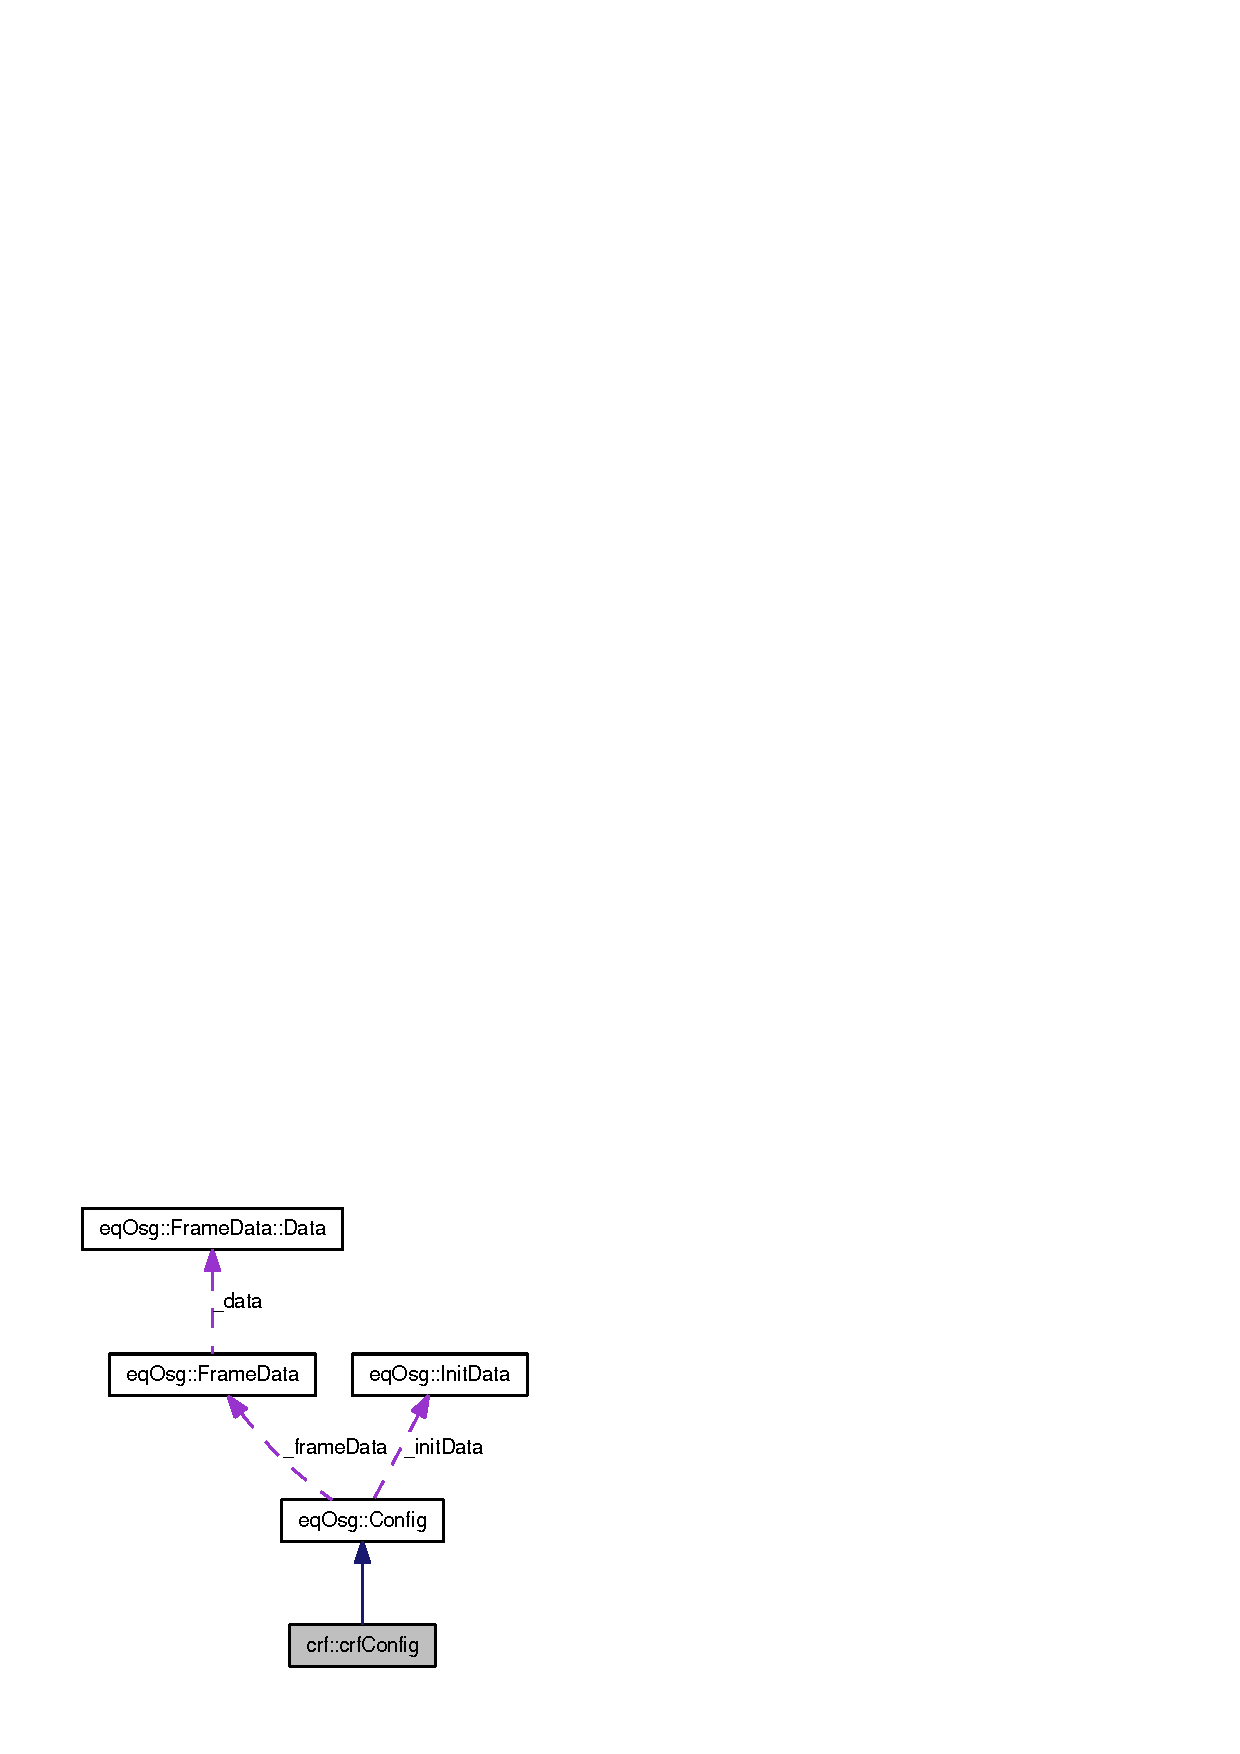
\includegraphics[width=257pt]{a00070}
\end{center}
\end{figure}
\subsection*{Public Member Functions}
\begin{CompactItemize}
\item 
\hyperlink{a00004_3ddcfcc9f305f6e8502078f922d7280f}{crfConfig} (eq::ServerPtr parent)
\item 
virtual bool \hyperlink{a00004_63938a0cf75d236b677c4cb147933b3c}{handleEvent} (const eq::ConfigEvent $\ast$event)
\begin{CompactList}\small\item\em Passes the desired events to the FrameData's event queue and calls the eqOsg::Config::handleEvents function. \item\end{CompactList}\item 
virtual uint32\_\-t \hyperlink{a00004_ebe9cfdff7f345f6d1f706be246520f7}{finishFrame} ()
\begin{CompactList}\small\item\em Clears the eventlist in FrameData and calls the base eq::Config::frameFinish(). \item\end{CompactList}\end{CompactItemize}


\subsection{Detailed Description}
This class extends the basic \hyperlink{a00045}{eqOsg} config class with support vor event forwarding to the pipe's viewer. 

\begin{Desc}
\item[See also:]\hyperlink{a00003}{eqOsg::Config} \end{Desc}


\subsection{Constructor \& Destructor Documentation}
\hypertarget{a00004_3ddcfcc9f305f6e8502078f922d7280f}{
\index{crf::crfConfig@{crf::crfConfig}!crfConfig@{crfConfig}}
\index{crfConfig@{crfConfig}!crf::crfConfig@{crf::crfConfig}}
\subsubsection[{crfConfig}]{\setlength{\rightskip}{0pt plus 5cm}crf::crfConfig::crfConfig (eq::ServerPtr {\em parent})\hspace{0.3cm}{\tt  \mbox{[}inline\mbox{]}}}}
\label{a00004_3ddcfcc9f305f6e8502078f922d7280f}


\begin{Desc}
\item[See also:]\hyperlink{a00003}{eqOsg::Config} \end{Desc}


\subsection{Member Function Documentation}
\hypertarget{a00004_ebe9cfdff7f345f6d1f706be246520f7}{
\index{crf::crfConfig@{crf::crfConfig}!finishFrame@{finishFrame}}
\index{finishFrame@{finishFrame}!crf::crfConfig@{crf::crfConfig}}
\subsubsection[{finishFrame}]{\setlength{\rightskip}{0pt plus 5cm}uint32\_\-t crf::crfConfig::finishFrame ()\hspace{0.3cm}{\tt  \mbox{[}virtual\mbox{]}}}}
\label{a00004_ebe9cfdff7f345f6d1f706be246520f7}


Clears the eventlist in FrameData and calls the base eq::Config::frameFinish(). 

\begin{Desc}
\item[Returns:]The finished frame's number. \end{Desc}
\begin{Desc}
\item[See also:]eq::Config::finishFrame \end{Desc}
\hypertarget{a00004_63938a0cf75d236b677c4cb147933b3c}{
\index{crf::crfConfig@{crf::crfConfig}!handleEvent@{handleEvent}}
\index{handleEvent@{handleEvent}!crf::crfConfig@{crf::crfConfig}}
\subsubsection[{handleEvent}]{\setlength{\rightskip}{0pt plus 5cm}bool crf::crfConfig::handleEvent (const eq::ConfigEvent $\ast$ {\em event})\hspace{0.3cm}{\tt  \mbox{[}virtual\mbox{]}}}}
\label{a00004_63938a0cf75d236b677c4cb147933b3c}


Passes the desired events to the FrameData's event queue and calls the eqOsg::Config::handleEvents function. 

\begin{Desc}
\item[Parameters:]
\begin{description}
\item[{\em event}]The to handle event. \end{description}
\end{Desc}
\begin{Desc}
\item[Returns:]True if the an event has been handled. \end{Desc}
\begin{Desc}
\item[See also:]eqOsg::Config::hanleEvent() \end{Desc}


Pass the mouse and keyboard events to framedata

Mouse events 

Reimplemented from \hyperlink{a00003_0ac41bd28010ff7f7638beb051b6c9b9}{eqOsg::Config}.

The documentation for this class was generated from the following files:\begin{CompactItemize}
\item 
E:/schule/Thesis/Repo/trunk/crf/src/crfConfig.h\item 
E:/schule/Thesis/Repo/trunk/crf/src/crfConfig.cpp\end{CompactItemize}
